\section{Methodology}

\subsection{Geometry Manipulation}
To simulate different geometry orientations, appropriate CAD must be produced with the rotated part.  To do this, Solidworks \cite{solidworks2024} was used.  This is the simplest way to generate new CAD from an existing model.
\newline \indent Solidworks has an Application Programming Interface (API) \cite{landry2022automatingSolidworksPython} that allows Visual Basic for Applications (VBA) to be passed from a Python script running on a computer into Solidworks.  Using this, a feature can be added to the existing feature tree of any part that is in the native Solidworks part format.  In the case of this project, the "Rotate" command can be added in to rotate a named part.
\newline \indent To export the part from Solidworks to a format that ANSYS can use, such as .step, another VBA command is used.  This one saves the part as a Step file.  A string can also be passed into the VBA script to change the naming of this file, which is useful for organization and file handling between scripts.
\subsection{Controlling a Simulation in ANSYS}
To automatically simulate LPBF in ANSYS, the PYMECHANANICAL and PYADDITIVE \cite{pymechanical2026} \cite{pyadditive2026} Python libraries can be used.  These libraries function as an API between Python and ANSYS.  Python needs to find or be shown the file path that contains the file that opens ANSYS Mechanical.  Once it has this, Python can open ANSYS and send commands into the opened instance of ANSYS.
\subsection{LPBF Simulation in ANSYS}
There is a caveat that LPBF residual stress simulation is not available in PYANSYS.  The workaround for this issue is to use a template file.  This is created by running an LPBF simulation, then saving it as a template file.  The original simulation is inconsequential and will be overwritten, but it is important that the original simulation is correct and complete.



\subsection{Algorithms}
To implement the algorithms mentioned in the research section, a higher level Python script must be used.  This high-level script controls the rotation and simulation scripts.  
\indent The first action this script takes is to run initial simulations.  The goal of these is to establish a baseline stress vs. orientation relationship for the searching algorithm to build off of.  For this simulation, a Sobol sequence is used.  As explained in Renardy et al., the Sobol sequence generates a quasi-random set of numbers.  \cite{Renardy2021Sobol}
\begin{figure}[H]
    \centering
    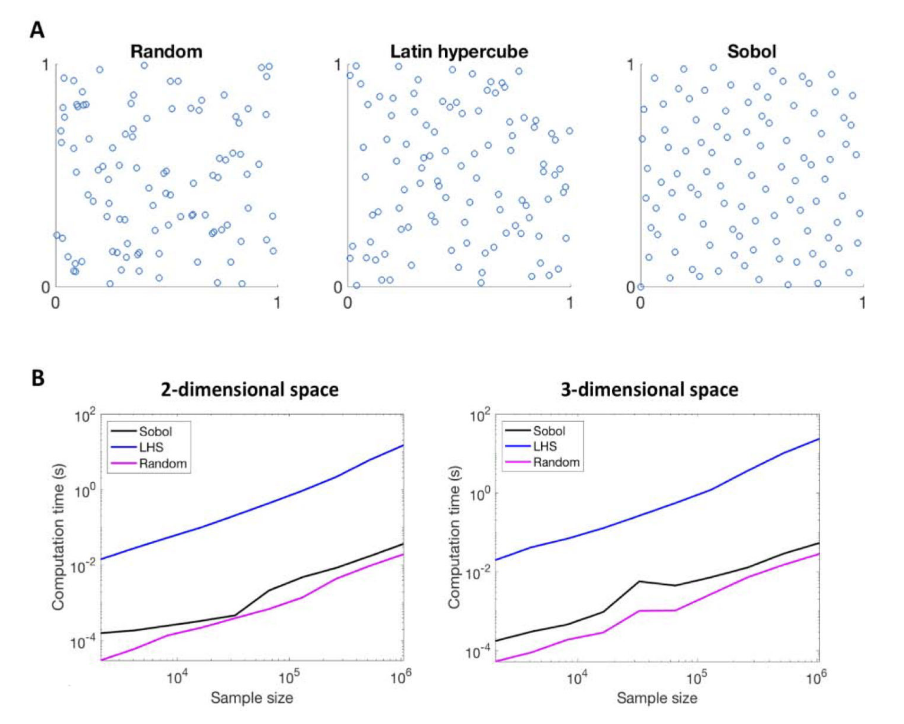
\includegraphics[width=5in]{Figures/Methodology/Sobol Comparison.png}
    \caption[Sobol Comparison]{Comparison of Sobol Sequence to other number generation methods \cite{Renardy2021Sobol}}
    \label{fig:Sobol Comparison}
\end{figure}

\indent In this instance, it is implemented via a Python library.  The Sobol Sequence gives a set of numbers (x,y,z) between 0 and 1.  Then the number is multiplied by 180 degrees to give an amount of rotation.  This is done for the first few “seed” simulations, which are designed to get the baseline for the simulation going.  The Sobol algorithm is used because of its capability for good coverage of the randomized space. Although this simulation takes place in the 3D space, ANSYS does its simulation layer by layer.  Meaning that everything along one Z-coordinate is taken as one step; raster angle does not matter.  Because of this, rotation about the Z-axis is removed, saving iterations and compute time. \cite{SciPySobol} 

\indent Once the initial stresses are known, the high-level script runs an algorithm to come up with new angles to simulate.  These angles are passed to the rotation script, and the rotated file is then simulated.  This cycle happens until the criteria for low residual stress is met.  Then the final angle is recorded, and the step file is to be printed.

\indent Gradient descent takes too many iterations, full contour optimization also takes too many iterations; it is Gaussian
A related study on optimization of prints was run by Menon et al..  In this paper, the computational expense of running simulations was, leading to the use of a Gaussian Process.  
\cite{Menon2022MultiFidelity}


\subsection{ANSYS LPBF Residual Stress Simulation}
According to the ANSYS LPBF Simulation Guide \cite{ansys_lpbf_simulation_guide_2025r1}, "The simulation is not meant to provide detailed thermal or structural results needed for prediction of micro-level process phenomena".  Thus, it is not meant for detailed looks at the crystal-level happenings of a part printed via LPBF.  
\newline \indent The LPBF simulation occurs following the same pattern as the printing of a part.  It starts at the build plate and builds the model up, layer by layer using "Standard element birth and death" \cite{ansys_lpbf_simulation_guide_2025r1}.  ANSYS doesn't simulate the scan path of the laser, as it "Would take enormous compute time making it impractical" \cite{ansys_lpbf_simulation_guide_2025r1}.  Instead, it applies heat to entire layers.  This saves compute time, while still giving an indication of the residual stress generated.  
\indent ANSYS lumps layers into "Super Layers" \cite{ansys_lpbf_simulation_guide_2025r1}, clumping layers together assuming that the layers are similar enough in profile that the heating effects will be similar between them.  These layers are heated as they are generated, and appropriate heat is retained in layers below to give the thermal gradients responsible for stresses.

\begin{table}[H]
  \centering
  \caption{Simulation parameters used in ANSYS LPBF simulations  \cite{ansys_lpbf_simulation_guide_2025r1}.}
  \label{tab:simulation-parameters}
  \begin{tabularx}{\linewidth}{|>{\raggedright\arraybackslash}p{2.5in}|>{\raggedright\arraybackslash}X|}
    \hline
    Parameter & Meaning \\
    \hline
    Base Geometry & Sets Print Base \\
    \hline
    Material & Material \\
    \hline
    Mesh Criteria - Mesh Method & Voxel, Tetrahedral, Cartesian \\
    \hline
    Supports & Sets up supports for the part \\
    \hline
    Heating Method & How is heat applied to a layer (Melting Temperature or Power) \\
    \hline
    Scan Time & Amount of time in layer \\
    \hline
    Beam Power & Power of Laser \\
    \hline
    Absorptivity & Fraction of laser power that goes into heating \\
    \hline
    Hatch Spacing & Space between scans \\
    \hline
    Deposition Thickness & Depth of powder per recoat \\
    \hline
    Scan Speed & Speed of scan \\
    \hline
    Dwell Time & Duration of pause between layers \\
    \hline
    Preheat Temperature & Starting temperature of build plate \\
    \hline
    Base Thermal Boundary Condition & Where the build plate is heated \\
    \hline
    Base Structural Boundary Conditions & Where base is fixed \\
    \hline
    Gas/Powder Temperature & Temperature of chamber and powder \\
    \hline
    Gas Convection Coefficient & Convection coefficient between new top layer and chamber gas \\
    \hline
    Powder Convection Coefficient & Effective convection coefficient from sides of build to powder bed \\
    \hline
    Powder Property Factor & Knockdown factor to estimate powder properties \\
    \hline
  \end{tabularx}
\end{table}

\indent The parameters and their descriptions in Table \ref{tab:simulation-parameters} are the values that are required to run this simulation as described in \cite{ansys_lpbf_simulation_guide_2025r1}.  These are the parameters that are to be set before running the LPBF simulation.  These values vary between alloy and printer, so it is important to get them right, or the simulation will be inaccurate to the print.

\begin{equation}[H]
\begin{bmatrix}
[M] & [0] \\
[0] & [0]
\end{bmatrix}
\begin{Bmatrix}
\ddot{u} \\
\ddot{T}
\end{Bmatrix}
+
\begin{bmatrix}
[C] & [0] \\
[C_{tu}] & [C_t]
\end{bmatrix}
\begin{Bmatrix}
\dot{u} \\
\dot{T}
\end{Bmatrix}
+
\begin{bmatrix}
[K] & [K_{ut}] \\
[0] & [K_t]
\end{bmatrix}
\begin{Bmatrix}
u \\
T
\end{Bmatrix}
=
\begin{Bmatrix}
F + [K_{ut}]\{T_{ref}\} \\
Q
\end{Bmatrix}
\label{eq:thermal-structural-coupled}
\end{equation}

Jung et al. \cite{jung2022numerical} use Equation \ref{eq:thermal-structural-coupled} to describe the background of what is happening in LPBF residual stress FEA.  It couples heating and cooling of the powder in the build to the expansion and contraction of the part being printed.  $[K^{ut}]$ is the thermoelastic stiffness matrix \cite{jung2022numerical}.  $[C_{tu}]$ is the attenuation matrix, and $[K^{t}]$ is the heat conduction matrix.  $[K^{t}]$ is found by adding $([K^{tb}])$ (Conductivity to material diffusion) and $([K^{tc}])$ (conduction based on the material convection surface).

\subsection{Geometry Modifications Necessary for Use}
There are several geometric and logistical requirements needed to prepare the geometry for simulation with this software.  For the AM simulation within ANSYS, both the part being printed and the print bed need to be present in the imported geometry.  In this simulation, it is required that they are named "base" and "part" with base being a flat rectangle, and part being what is being printed.  This is necessary for Solidworks to identify which part to move, and for ANSYS to find which part to simulate.  The rectangular base must have its bottom face (away from part) located at z=0.  This is so a fixed constraint can be applied to constrain movement degrees of freedom during the mechanical simulation.  The part must be offset in the z from the build plate to allow for supports to be built, otherwise the part will be stuck to the build plate, and its geometry will be affected during the wire EDM separation of part from build plate.